\documentclass{aastex631}
\usepackage[utf8]{inputenc}
\usepackage{graphicx}
\usepackage{amsmath,amssymb}
\begin{document}
\title{On the Dynamics of Planetary Systems in Embedded Cluster Environments}
\author{Elizabeth A. Ellithorpe}
\date{Spring 2021}


%\maketitle
%\begin{center}
%
\includegraphics[width=0.6\textwidth]{fig/ou_seal.jpg}
%\end{center}

\newpage
\begin{abstract}
    Using numerical simulations of s-type gas giants orbiting within a binary stellar pair that is integrated simultaneously with an embedded stellar cluster 
    environment, we find that the orbital evolution of the binary companion, when perturbed by the cluster, can affect the stability of the planets within its orbit.
    We present several initial findings that characterize both the behavior of the binary companion during a planetary 
    disruption event as well as the markers that such an event leaves behind on surviving planets. We note the importance of the inclusion
    of the cluster environment in these simulations as interactions between the binary and cluster stars are the main driver
    in planetary instability. Destabilized planetary systems ultimately end with significantly different orbital parameters for the 
    surviving planets as compared to systems the retain all 4 of the original gas giants. The altered orbital configuration of 
    surviving planets in a destabilized system point to a dynamical source of exoplanets that have a 
    spin-orbit misalignment with their host star. 
\end{abstract}

\section{Background \& Motivation}
\indent The dynamics of planetary systems serve as signposts of their formation and subsequent evolution. Thus the study of dynamical modeling 
of exoplanets is a form of archaeology: using both observations and simulations of existing stable planets, we can walk back in 
time to discover which physical processes govern the behavior of extrasolar worlds.  Dynamics offers a strong union of computational 
and observational astronomy, where an influx of exoplanet observational data has dovetailed nicely with a surge in advancements in numerical algorithms
over the last two decades. \\
\indent It has been long thought that most stars spend some of their early lives in a cluster environement, a large scale sphere of gas that acts as a stellar nursery
 that condense into pre-stellar cores in the gas and dust (\cite{lad03}). Recent work(\cite{sad17}) has also bolstered the theory(\cite{kro95}) that the majority of stars 
 are born in a stellar multiple is true, where their dense pre-stellar cores mutually bound together in a dusty envelope. 
 These multiple bound cores, likely formed
 via fragmentation (\cite{bon94},\cite{bat03},\cite{tur09}) either stay together in a binary as interactions with their gaseous
 disk decrease the separation between the pair (\cite{bat00},\cite{bat03}), or are pulled apart by a cluster environment(\cite{kro01}). 
 %Dynamical interactions from a stellar cluster have also been shown to effect the orbital architecture of existing binaires. 
 While clusters can unbind so-called 'soft binaries'(\cite{kro01}), dynamical interactions with a cluster are not sufficient to explain the observed
 period distribution of binary stars. Thus, their nascent orbital architecture results from the fragmentation process and interactions with a circumstellar disk
 early on in their lives (\cite{krobur01}), and should be considered when we discuss the formation and the dynamics of planets in a holistic manner.\\
 %Planet formation likely occurs via the same pathways in binary populations as it does around single stars(\cite{bat11}). 
 %The ubiquitous nature of both stellar multiples and stellar clusters necesscitate their inclusion in discussions of planetary dynamics. 
 \indent While planets in a binary system have been 
 previously studied in depth with N-Body integration, the binary that interacts with the planets is for the most part unperturbed by outside forces 
 (i.e., \cite{hol99},\cite{hag07}),
 or, if the binary is modeled in a cluster, planets are not included (i.e. \cite{krobur01}). Similarly, planetary systems as they might interact with a cluster environment
 have been modeled, but often with mock fly-bys of a star rather than a fully evolved cluster (i.e., \cite{rec09},\cite{cat20}). A union of these two simultaneous phenomena,
 a binary's effect on planets and a cluster's effect on a binary, are necesscitated by the ubiquitous nature of these interactions in young systems. With N-Body simulations
 produced by hybrid symplectic integration scheme, we offer a new perspective at this complex problem. 
\subsection{Previous Work}
The presence of a binary companion has been considered in studies of planetary formation since the 1960's. Early treatments of planetary stability in a binary system worked
within the framework of the restricted 3-body problem (\cite{hua60}) and numerical estimates based on analytic models (\cite{hep78}). Early work established that 
both the formation and the stability of planets in a binary system was possible.\\
Later on, numerical integration to evolve these systems began in earnest, owing largely to developments in symplectic integration methods (such as the work described 
by \cite{wis91}) that 
allowed for efficient integrations of entire planetary systems in the presence of a binary. The main question that arises in such a system is in what cases does a binary 
companion preclude the existence of stable planets. An early work that used the Wisdom-Holman scheme is the exploration of the Alpha Centauri system in \cite{wie97},
in which the authors use N-Body integrations in the \cite{wis91} scheme to assess the stability of test particles in and around the Alpha Centauri triplet. \\
The seminal works in the field of planetary stability in a binary system are \cite{dvo86} and \cite{hol99}. \cite{dvo86} looked at integrating systems of test
particles in the
the restricted 3-body problem with the Lie series method (Delva 1985) and established an upper and lower critical orbit that began mapping a region of stability 
for a planet based on the eccentricity of the binary system. \cite{dvo86} looked at various eccentricities of the binary companion, but in all cases the mass of the binary and 
the central star were the same. 
 Holman \& Wiegert further built upon this stability analysis via symplectically integrating binary systems 
with both p-type and s-type planets. Their integration work, based on the Wisdom-Holman method,
 produced an analytic form of a planet's critical orbit based on both the eccentricity of the binary and the mass
ratio $\mu = \frac{M_{bin}}{M_{primary}}$. Also drawing on \cite{wis91} is the work described in \cite{ina97}, in which the solar system is integrated in the presence of a 
binary. The authors exemplify the Kozai effect (\cite{koz62}) in which an inclined binary exchanges angular momentum with the planets, and also show that the planets evolve in concert 
as a rigid disk. This work revealed that the Kozai effect is a pathway that can lead to increased eccentricity of planets. Another analysis of the Kozai effect on planetary stability that 
takes a different, secular approach is \cite{fab07}, in which the authors integrate the motion of planets in the presence of a binary to show that tidal friction can circularize an 
orbit made eccentric by an inclined binary companion.\\
The stability analysis of Holman \& Wiegert remains of interest to this day, with recent work such as \cite{lam18} further refining
their original critical orbit with a neural network and integrations performed in the publically available REBOUND integrator.
 Analysis of planets in binaries continue with work 
in \cite{cha02} in which the authors use a mixed variable symplectic method to analyze planetary accretion both in a system where the test planet orbits a primary and 
is perturbed by a distant binary and one in which the planet orbits around the binary system in its entirety. While \cite{cha02} utilizes an integrator that allows for the presence 
of a binary, further work by \cite{beu03} introduces a symplectic scheme based on the \cite{wis91} method, called Hierarchical Jacobian Symplectic, that allows for the 
integration of a multiple system of any size (i.e., numbering more massive bodies than just a binary) as long as there is a retained
hierarchy among the masses.  \\
The presence of a distant companion has also been considered in numerical integrations of protoplanetary (debris) disks. \cite{rec09} use the HJS scheme (\cite{beu03}) 
to integrate the HD141596 triple star system and debris disk in the presence of stellar flybys. 
\cite{beu14} used symplectic integration to model the Fomalhaut triplet in addition to its dust belt.  \\

\indent On the larger scale, N-body simulations of stellar clusters have been used to study how stellar binaries interact with a cluster environment. \cite{bat03} 
use high resolution simulations of a collapsing gas cloud to to study the fragmentation of gas into dense cores, 
and the subsequent evolution of these young stars into binaries. They find that very
 tight binaries are formed by the hardening of wider binaries via dynamical interactions. \cite{ada06} and \cite{pro09} used N-Body simulations of moderately sized stellar clusters
  (100-10,000 members) or embedded clusters to study the impact of a cluster environment on planet formation, particularly in how protoplanetary disks may be affected by stellar raditation.
  They find that disruption of model solar systems in an evolved cluster environment(\cite{ada06}) should be relatively rare due to the paucity of encounters between a 'solar system' 
  in question and a passing star, but in younger, denser clusters the photoevaporation of disks by a cluster environment can be appreciable(\cite{pro09})
  
  \cite{hao13} takes a monte carlo approach to simulating planetary systems in an
 open cluster to explore planet-planet scattering. The authors model a stellar flyby and find that multi-planet systems are more sensitive to an open cluster 
 environment that single planet system. In the realm of exploring planetary orbits in clusters via a model stellar fly-by is work by \cite{mal11} and \cite{bre19}.
  \cite{mal11} shows that fly-bys increase the chance of planetary ejection, while \cite{bre19} shows that a cluster
star can create a retrograde planetary orbit.  \\

In summary, while there is an extensive body of work on the integration of planets in a binary system and the evolution of planets in a cluster environment, previous work
largely assumes that the binary is in isolation and does not evolve due to external forces; work concerning cluster environments either model interactions as a flyby 
or do not include a simultaneous binary system. The work we present here is novel in its approach in that it allows the binary companion to be altered by a cluster environment,
and that we fully model the cluster rather than taking a fly by apporach. 
\subsection{Numerical Integration}
To achieve such a broad assortment of work on the dynamics of stars and planets, astronomers have turned to both N-Body and hydrodynamic simulations as the workhorses
of their experiments.
In particular, symplectic integration schemes have been popular as they have largely reduced error in energy over time and are 
faster than other N-body algorithms(\cite{cha99},\cite{sah92}).
This is due to the formulation of advancing the positions and momenta of bodies via Hamilton's equations, which preserve inherently 
both energy and angular momentum. In using a
symplectic scheme, the Keplerian nature of the orbits of small bodies about a large central mass can be 'built in' to the Hamiltonian, allowing for very fast integrations
of situations like the solar system, where the planets are on Keplerian orbits and are not undergoing close encounters with another. 
Therein we run into our first problem with early symplectic schemes: to investigate the dynamics of celestial bodies, we need to allow for close approaches
that could kick bodies off their Keplerian paths. An additional problem that must be considered is that, unlike traditional integration methods,
the preservation of phase space in symplectic schemes is dependent on a permanent choice of time step (\cite{lee97conf}).
%Additionally, pure symplectic integrators do not allow for adaptively sized time steps (\cite{lee97conf}), making
%the choice of timescale for integrations  \\
\cite{wis91} is the seminal work in introducing a  scheme known as a \textit{mixed variable symplectic} (MSV) integrator. Such a scheme can quickly integrate
a system with a hierarchical composition (i.e., the Keplerian motion of the planets is a much larger part of the Hamiltonian that perturbations from a distant star).
\cite{sah94} showed that the limitation of a fixed timestep could be partially overcome by assigning a different timestep to different bodies in an integration. This
can lead to an increase in efficiency for systems in which bodies have different orbital periods and therefore require different timescales. 
\indent Some early applications of these MVS integrators include \textit{SyMBA} described in \cite{dun98} and the \textit{Mercury} 
integrator by \cite{cha99}. SyMBA addresses the inability of symplectic integrations to change the value of timesteps via judicious splitting of the Hamiltonian,
in which strong perturbative terms have comparatively smaller timesteps(\cite{dun98}). \cite{cha99} cites this choice as difficult to implement, and instead 
took a hybrid approach in the creation of \textit{Mercury}. \\
 \textit{Mercury} was a similar advancement to \textit{SyMBA} in the field of planetary dynamics in that it was a \cite{wis91} scheme that retained the advantages of a symplectic scheme 
(i.e., no build up of error in energy except due to numerical round off) but allowed for close encounters between bodies. \textit{Mercury} and previous work by \cite{sah94}
addressed the adaptive time step issue by allowing disparate bodies in the integration to have different time steps, as long as those assigned time steps 
did not change during the course of the integration. This is useful for instance if a modeled planetary system
has bodies with very different orbital periods.
Still, the need for adaptive time steps can be seen in the case of a close approach between
two bodies where the characteristic timescale of the encounter can be quite a bit smaller than the original time steps. 
%Instead of requiring symplectic schemes
%with close approaches to have prohibitively small time steps, the idea of a hybrid symplectic integrator came about. 
In \textit{Mercury} and other integrators (\cite{dun98},\cite{ric00}), the Hamiltonian that describes
can be split and integrated separately(\cite{yos90},\cite{sah92}). In \textit{Mercury}, it is split into a Keplerian portion, which for most of the 
integration is the largest portion, and an interaction part that dominates when two bodies 
approach one another. As the interaction part is normally small except when two bodies are close, the Keplerian part of the Hamiltonian is comparably large and can be solved
analytically, greatly increasing the speed of the integrator. \\
\indent A change came to the \textit{Mercury} code as authors(\cite{cha02}) then turned to the next problem: the inclusion of additional massive bodies, such as a 
binary companion, that interact with the planetary system. \cite{cha02} marked the inclusion of a hierarchical coordinate system
% \textit{democratic heliocentric} coordinate system(\cite{dun98}) 
to allow for an additional massive body in the Hamiltonian. These coordinates allow for different time steps to be used for concentric shells around the primary star,
such that planets orbiting the primary can have different integration time steps.
The numerical integrator we use for this work is built on the foundation of the original \textit{Mercury} package but with changes
to allow the inclusion of multiple bound massive bodies (i.e., a binary or triplet star system) and unbound massive bodies (i.e. stars in a cluster environment)(\cite{kai17}).
The integration of the planetary system around the primary. We still use the democratic heliocentric coordinates for the planetary system, but the binary
is defined relative to the center of mass of the planetary system, and the cluster stars are defined simply with their inertial coordinates. By letting the different
bodies be treated with different coordinate system, this version of \textit{Mercury} retains the advantages of a pure symplectic integrator while still being able 
to evolve the unbound cluster stars. That is, there is not a build up of energy error, the Keplerian nature of the planetary system (while not undergoing a close approach)
is retained, and simultaneously the cluster stars and their close approaches can be integrated efficiently in a leapfrog-like scheme. \\
\indent These changes to \textit{Mercury} are crucial to realistic modeling of binary-planet systems in a stellar cluster.
 In this work we are largely concerned with the overall fate of binary systems and their planets during interactions with the cluster. Moreover, our
work has also revealed some intriguing changes in orbital architecture of planetary systems that have a close encounter with an excited binary companion.
%\indent The inclusion of both the binary and the cluster environment in our simulations opens the door to exploring many existing question in planetary dynamics. One
%such question that will be addressed in this work is the misalignment of the spin-orbit angle of gas giants with their host star. In particular, exoplanet observations
%have indicated that hot jupiters have a stronger likelihood to be on an inclined orbit relative to the spin axis of the central star. Hot jupiters are thought to have
%undergone significant dynamical migration to end up so close to their host stars, as gas giants must form beyond the snow line of a system for their 
%cores to gain sufficient mass. It has been proposed that interactions with a distant binary companion could drive this migration. 
%\indent One such union of observation and simulations that makes up the basis of motivaiton for this work is the prevalence 
%of highly inclined gas giants on very close orbits known as \textit{hot jupiters}. This work points to the potential that these inclined 
%hot jupiters may in fact arise from dynamical interactions with a distant binary companion in cluster environments. \\
%While hot jupiters are indeed a system of keen interest from exoplanet astronomers, there are other interesting architectures that
%this numerical work can be used for. For instance, we now know that the majority of the exoplanet population consists of so called 
%\textit{super earths} that fall between the size of Earth and Neptune, covering the range between $1.5 R_{earth}$ and $2 R_{earth}$.
%Their higher mass than terrestrial planets points to formation that could be either within or beyond the snow line of their host systems,
%which hints toward some very interesting dynamical evolution for these planets. One such super earth system with an orbital misalignment
%is that of $\pi$ Mensae. The mutual inclination between observed exoplanets like $\pi$ Men c and the spin of their host star, measured via
%the Rossiter-McLaughlin effect\cite{hod21} indicates
%a dynamical history that must be understood to have a full picture of exoplanet formation.
\section{Methods}
\subsection{Numerical Intergration}
This work is produced by a hybrid symplectic integrator that modifies the public version of \textit{Mercury} such that we can simultaneously evolve a system of planets
in the presence of a bound binary companion that is in turn interacting with a large scale embedded stellar cluster.
In this scheme, we define 3 distinct types of bodies: planets 
bound to the primary, the binary companion, and cluster stars. The cluster star positions are treated with their inertial coordinates,
measured only with respect to the origin. The binary's position
is integrated with respect to the center of mass of the primary star system. 
The planets are integrated purely with respect to the primary star.
The choice of these coordinates means that the cluster stars are integrated with a purely symplectic $T+V$ leapfrog scheme. This
conserves energy and angular momentum, and is quite accurate as the timescale of cluster stars orbiting in the cluster
is much larger than the characteristic timescale set by the orbits of the planetary bodies. The binary and the planets 
are also integrated symplectically, although with a mixed variable symplectic Wisdom-Holman scheme(\cite{wis91}). Finally, when close encounters do occur in the simulations,
a change is made to integrate these directly with a Bulirsch-Stoer scheme with a much smaller time step than was used prior to the close
encounter. Thus, this scheme largely preserves the useful angular momentum and energy conservation of a symplectic scheme while allowing
for close encounters.
Equation \ref{positions} shows how we define the position of each type of object, where $\vec{X}_A$ represents the position of the primary star,
$\vec{X}_B$ the position of the binary, $X_{i}$ for $1\leq i \leq N_P$ is the position of a planet, and $\vec{X}_i$ for $N_P < i \leq N_P+N_S$ is the position of a cluster star.
The lowercase $\vec{x}$ represents each type of body's inertial coordinates relative to the origin/center of mass of the cluster.

\begin{equation}
    \begin{split}
        \vec{X}_A = \frac{m_a\vec{x}_A+m_B\vec{x}_B+\sum_{j=1}^{N_P}m_j\vec{x}_j}{m_A+m_B+\sum_{j=1}^{N_P}m_j} \\
        \vec{X}_i = \vec{x}_i-\vec{x}_A \text{   for   } 1\leq i \leq N_P \\ 
        \vec{X}_B = \vec{x}_B-\frac{m_A\vec{x}_A+\sum_{j=1}^{N_P}m_j\vec{x}_j}{m_A+\sum_{j=1}^{N_P}m_j} \\
        \vec{X}_i = \vec{x}_i \text{   for   } N_P < i \leq N_P+N_S
     \end{split}
\label{positions}
\end{equation}
As such, we define some useful position vectors for changing between reference frames.
\begin{equation}
\begin{split}
    \vec{s} = \frac{\sum_{i-1}^{N_P}m_i\vec{X}_i}{m_A+\sum_{i-1}^{N_P}m_i}\\
    \vec{\Delta} = \vec{X}_A-\frac{\sum_{i=1}^{N_P}m_i\vec{X}_i+m_B(\vec{X}_B)+\vec{s})}{m_A+m_B+\sum_{i=1}^{N_P}m_i}
\end{split}
\end{equation}

In this symplectic scheme, we must consider how Hamilton's equations evolve for all members of the system. We consider mutual gravitation
between the primary star, binary star, planets and cluster stars. We also consider the gravitational tide from the gas of the 
Plummer potential(\cite{plu11}) that we assume to be binding the cluster stars together. I will include the derivation for the Plummer potential here.
This force from the Plummer potential is dependent on the inertial position of each massive body within the cluster, which can make the 
calculation in our chosen coordinates fairly complicated. The expression for the force from the sphere of gas is different for each type of body,
namely the planets, the binary, and the cluster star. We begin with the expression for the mass distribution of a Plummer sphere in inertial coordinates. 
\begin{equation}
\rho (\vec{x}) = \frac{3M_0}{4\pi a_0}+\biggl(1+\frac{|\vec{x}|^2}{a_0^2} \biggr)^{-5/2}
\end{equation}
This mass distribution, where $M_0$ is the total mass in gas of the Plummer sphere and $a_0$ is a scale parameter that sets the size of the flat core region results
in a gravitational potential of:
\begin{equation}
    \Phi(\vec{x}) = \frac{GM_0}{(|\vec{x}|^2+a_0^2)^{1/2}}
\end{equation} 
The potential energy of our system can then be written as:
\begin{equation}
    \begin{split}
        V_{Plum} = \sum_{i=N_p+1}^{N_p+N_s}\frac{GM_{gas}m_i}{(X_i^2+a_0^2)^{1/2}} + 
        \sum_{i=1}^{N_p}\frac{GM_{gas}m_i}{(|(\vec{\Delta}+ \vec{X_i})|^2+a_0^2)^{1/2}} \\ 
        +\frac{GM_{gas}m_B}{(|(\vec{\Delta} + \vec{s} + \vec{X}_B)|^2+a_0^2)^{1/2}} 
        + \frac{GM_{gas}m_A}{(|\vec{\Delta}|^2+a_0^2)^{1/2}} 
    \end{split}
\end{equation}
For clarification, the inertial position with which the strength of the Plummer potential is measured in simulation coordinates is $\vec{X}_i$ for the cluster stars,
$\vec{\Delta}+\vec{X}_i$ for the planets, $\vec{\Delta}+\vec{s}+\vec{X}_B$ for the binary, and $\vec{\Delta}$ for the primary.
We can then calculate the acceleration due to the Plummer sphere on each body(indexed with $i$) for each cartesian coordinate (indexed with $u$) via:
\begin{equation}
    m_i\frac{dv_{i,u}}{dt} = \frac{\partial V_{plum}}{\partial x_{i,u}}
\end{equation}
\subsubsection{Cluster Stars}
The positions of the clusters stars in the integration coordinates are exactly their inertial coordinates in this integration scheme 
(i.e., they are measured relative to the origin). This makes finding the acceleration due to the Plummer tide much more straightforward 
than for the planets and the binary star pair.
\begin{equation}
    \vec{X}_i = \vec{x}_i \text{  for  } i>N_p+1
\end{equation}
\begin{equation}
    m_i\frac{dv_{i,u}}{dt} = -\frac{\partial V_{Plum}}{\partial X_{i,u}}
\end{equation}
\begin{equation}
    \frac{dv_{i,u}}{dt} = \frac{-1}{m_i}\sum_{k=N_p+1}^{N_p+N_s}\frac{GM_{gas}m_kX_{k,u}delta_{ik}}{(|\vec{X}_k|^2+a_0^2)^{3/2}} = 
    \frac{-GM_{gas}X_{i,u}}{(|\vec{X_i}|^2+a_0^2)^{3/2}}
\end{equation}
We can see that the acceleration due to the Plummer sphere on the cluster stars is simply a direct term based on the mass of the gas 
enclosed by the cluster star's current position.
\subsubsection{Planets}
\begin{equation}
    m_p\frac{dv_{i,u}}{dt} = -\frac{\partial V_{Plum}}{\partial X_{i,u}}
\end{equation}
Recall that $\Delta$ is a function of the position of the planets. The relevant partial here is:
\begin{equation}
\frac{\partial \Delta}{\partial X_i} = \frac{\partial X_A}{\partial X_i} - 
\frac{\sum_{k=1}^{N_P}m_k\frac{\partial X_k}{\partial X_i}+m_B\frac{\partial}{\partial X_i}(X_b+s)}{m_A+m_B+\sum_{k=1}^{N_p}m_k}
\end{equation}
\begin{equation}
   \frac{\partial \Delta}{\partial X_i} = 
   -\frac{\sum_{k=1}^{N_p}m_i\delta_{ik}+m_b\frac{\delta s}{\delta X_i}}{m_A+m_B+\sum_{k=1}^{N_p}m_k} 
\end{equation}
\begin{equation}
\frac{\partial \Delta}{\partial X_i} = 
\frac{-m_i-m_b\frac{m_i}{m_A+\sum_{k=1}^{N_P}m_k}}{m_A+m_B +\sum_{k=1}^{N_P}m_k}
\end{equation}
\begin{equation}
    \frac{\partial \Delta}{\partial X_i} = -m_i\frac{1}{m_A+\sum_{k=1}^{N_P}m_k}
\end{equation}
\\ \\
\begin{equation}
\begin{split}
    \frac{dv_{i,u}}{dt} = 
    \frac{-GM_{gas}}{m_i}\frac{\partial}{\partial X_{i,u}}\biggl(\sum_{k=1}^{N_P}\frac{m_k}{\sqrt{|\vec{\Delta}+\vec{X}_i|^2+a_0^2}}\\
    +\frac{m_A}{\sqrt{|\vec{\Delta}|^2+a_0^2}}+\frac{m_B}{\sqrt{|\vec{\Delta}+\vec{s}+\vec{X}_B|^2+a^2_0}} \biggr )
\end{split}
\end{equation}
\begin{equation}
    \begin{split}
    \frac{dv_{i,u}}{dt} = 
    \frac{-GM_{gas}}{m_i}\biggl(\sum_{k=1}^{N_P}\frac{-m_k(\Delta_u+X_{k,u})}{(|\vec{\Delta}+\vec{X_k}|^2+a_0^2)^{3/2}}(\frac{\partial \Delta}{\partial X_i}+
    \frac{\partial X_k}{\partial X_i})\\+\frac{m_A\Delta_u}{(|\vec{\Delta|^2}+a_0^2)^{3/2}}\frac{m_i}{m_A+\sum_{k=1}^{N_p}m_k} \biggr)    
    \end{split}
\end{equation}


\begin{equation}
    \begin{split}
      \frac{dv_{i,u}}{dt} = 
      \frac{GM_{gas}}{m_A+\sum_{j=1}^{N_P}m_j}\biggl(\sum_{k\neq i}^{N_P}\frac{m_k(\Delta_u+X_{k,u})}{(|\vec{\Delta}+\vec{X_k}|^2+a_0^2)^{3/2}}+ 
      \frac{m_A\Delta_u}{(|\vec{\Delta}|^2+a_0^2)^{3/2}} \biggr)\\+
       \frac{GM_{gas}(\Delta_u+X_i)}{(|\vec{\Delta}+\vec{X_i}|^2+a_0^2)^{3/2}}\biggl(\frac{-m_i}{m_A+\sum_{j=1}^{N_P}m_j}+1\biggr)
    \end{split}
\end{equation}


\begin{equation}
    \begin{split}
    \frac{dv_{i,u}}{dt} = 
    \frac{GM_{gas}}{m_A+\sum_{j=1}^{N_P}m_j}\biggl(\sum_{k=1}^{N_P}\frac{m_k(\Delta_u+X_{k,u})}{(|\vec{\Delta}+\vec{X_k}|^2+a_0^2)^{3/2}}+
    \frac{m_A\Delta_u}{(|\vec{\Delta}|^2+a_0^2)^{3/2}} \biggr)\\ - \frac{GM_{gas}(\Delta_u+X_i)}{(|\vec{\Delta}+\vec{X_i}|^2+a_0^2)^{3/2}}   
    \end{split}
\end{equation}

\subsubsection{Binary Companion}
The coordinate $\Delta$ is also a function of the position of the binary. Here the useful partial to calculate is:
\begin{equation}
    \frac{\partial \Delta}{\partial X_B} = \frac{-m_B}{m_A+m_B+\sum_{i=1}^{N_P}m_i}
\end{equation}
\begin{equation}
    \begin{split}
        \frac{dv_{B,u}}{dt}=\frac{1}{m_B}\frac{\partial V_{Plum}}{\partial X_{B}}
\end{split}
\end{equation}
\begin{equation}
    \begin{split}
        \frac{dv_{B,u}}{dt}=\frac{-GM_{gas}}{m_B}\biggl(\sum_{k=1}^{N_P}\frac{\partial}{\partial X_{B}}\frac{m_k}{(|\vec{\Delta}+\vec{X_k}|^2+a_0^2)^{1/2}} \\
        +\frac{\partial}{\partial X_B}\frac{m_B}{(|\vec{\Delta}+\vec{s}+\vec{X_B}|^2+a_0^2)^{1/2}}+\frac{\partial}{\partial X_{B}}\frac{m_A}{(|\vec{\Delta}|^2+a_0^2)^{1/2}} \biggr)
    \end{split}
\end{equation}

\begin{equation}
    \begin{split}
        \frac{dv_{B,u}}{dt}=\frac{-GM_{gas}}{m_B}\biggl(\sum_{k=1}^{N_P}\frac{m_k(\Delta+X_k)\frac{\partial}{\partial X_B}(\Delta+X_i)}{(|\vec{\Delta}+\vec{X_k}|^2+a_0^2)^{3/2}} \\
        +\frac{m_B(\Delta+s+x_B)\frac{\partial}{\partial X_B}(\Delta+s+X_B)}{(|\vec{\Delta}+\vec{s}+\vec{X_B}|^2+a_0^2)^{3/2}}+\frac{m_A\Delta\frac{\partial \Delta}{\partial X_B}}{(|\vec{\Delta}|^2+a_0^2)^{3/2}} \biggr)
    \end{split}
\end{equation}

\begin{equation}
    \begin{split}
        \frac{dv_{B,u}}{dt}=-GM_{gas}\biggl(\sum_{k=1}^{N_P}\frac{-m_k(\Delta_u+X_{k,u})}{(|\vec{\Delta}+\vec{X_k}|^2+a_0^2)^{3/2}}\frac{1}{m_A+m_B+\sum_{k=1}^{N_P}m_k} \\ 
        + \frac{(\Delta_u+s_u+X_{B,u})}{(|\vec{\Delta}+\vec{s}+\vec{X_B}|^2+a_0^2)^{3/2}}\bigl(1-\frac{m_B}{m_A+m_B+\sum_{k=1}^{N_P}m_k}\bigr)\\+\frac{-m_A\Delta}{(\vec{\Delta}|^2+a_0^2)^{3/2}(m_A+m_B+\sum_{k=1}^{N_P}m_k)}\biggr)
    \end{split}
\end{equation}
\begin{equation}
    \begin{split}
        \frac{dv_{B,u}}{dt} = \frac{GM_{gas}}{m_A+m_B+\sum_{j=1}^{N_P}m_j}\biggl(\sum_{k=1}^{N_P}\frac{m_k(\Delta_u+X_{k,u})}{(|\vec{\Delta}+\vec{X}_k)|^2+a_0^2)^{3/2}}\\ 
        + \frac{X_{B,u}+s_u+\Delta_u}{(|\vec{\Delta}+\vec{X}_B+\vec{s}|^2+a_0^2)^{3/2}} +\frac{m_A\Delta_u}{(|\vec{\Delta}|^2+a_0^2)^{3/2}}\biggr) - 
        \frac{GM_{gas}(X_{B,u}+s_u+\Delta_u)}{(|\vec{\Delta}+\vec{X}_B+\vec{s}|^2+a_0^2)^{3/2}}
    \end{split}
\end{equation}
\subsection{Experimental Design}
First, we must decide how to build our stellar clusters. The masses of the stars are sampled from the Charbrier (2003) piecewise IMF (\cite{cha03}) where we set
an upper mass limit of $150 M_{\odot}$(\cite{wei04}).
The positions of the stars are sampled via weights assigned from a Plummer distribution of gas (\cite{plu11}). We are therefore assuming that the stars
condense out of mass in a spherical Plummer potential. The mass of the Plummer sphere that acts as the gaseous environment for the
embedded stars is chosen assuming a $10\%$ star formation efficiency. Then, the virial speeds of each star are calculated based on their position
and we assign them a random initial velocity vector at $8\% v_{virial}$\cite{lev10}. Once the cluster is constructed, we generate $100$ simulations
where for each simulation a random cluster star is assigned the role of the primary. As these simulations are run in democratic heliocentric
coordinates, all other stars are redefined with respect to the rest frame of the primary. A set of 4 gas giants, analogous to the orbits and 
masses of Jupiter, Saturn, Uranus, and Neptune, are set around the primary, and a coplanar binary companion with eccentricity of 
$0.5$ is added. The eccentricity was chosen to match observations of relatively wide (greater
than 50au separation) binaries(\cite{tok16}), although the eccentricities of these systems are not well constrained. Future work will include
analysis of other initial binary eccentricity choices, ensuring that the choices are stable in isolation.
The binary takes on a range of semi-major axis values between $300$au and $800$au. We intially tested
a range of $100$ to $1e4$au, but found that approximately closer than $300$ au and the planets are unstable, and outside $800$au 
the binary is very quickly stripped away by the cluster and therefore no longer interacts meaningfully with the planets. 
 All of these systems in the final range of binary semi-major axis were verified via numerical integration to be inherently stable for $10 Myr$ when \textit{not} 
 in the presence of a stellar cluster. \\
\indent To design the parameters of the stellar cluster, we look to the catalog compiled by Lada \& Lada (2003)\cite{lad03}. The majority of clusters in the catalog have a mass less than
$200M_{\odot}$ and a number of stars less than $250$. To model these most common clusters, we created two suites of simulations, one with a total mass of $80M_{\odot}$ and one
with a mass of $160 M_{\odot}$. The smaller $80M_{\odot}$ cluster had $122$ stars and the larger $160 M_{\odot}$ has $221$. For good measure, we created a third larger cluster
that mimics the observed characteristics of the embedded Monoceros R2 cluster, with a mass of $341 M_{\odot}$ and $509$ stellar cluster members(\cite{car97}). \\
The time step of our simulations is set to $100$ days, sufficiently small for the orbital periods of the gas giants. 
%The simulations were run on the OU supercomputing cluster \textit{Schooner}.
%\section{Stellar Clusters and the Birth Environment of Planets}
%It is now thought that the majority of stars form in a nascent multiple, spending their early stages of life gravitationally bound to a 
%binary or triplet companion. This adds a layer of complexity to the challenge of accurately simulating planetary systems, as it is likely 
%that planets will have spent some of their life in the presence of a stellar companion. To add an even further layer of dynamics, stars form 
%in the hundreds in cluster environments, adding distant stellar perturbations as well as the gravitational tides of gas and dust to our list 
%of physics to model. Through the use of a symplectic integrator built on the bones of the \textit{Mercury} (1999) code, we look to model the 
%dynamics of toy planetary systems in stellar cluster environments, ranging from $80 M_{\odot}$ to $341 M_{\odot}$ in total mass. These sample
%some of the smallest to some of the largest embedded cluster environments.\cite{lad03} 
\section{The Fate of Binary Systems}

\subsection{Characteristics of Destabilization}
First, we will take a holistic look at all simulations that undergo planet loss. In total, we see than $\approx 6\%$ of our simulations
have a planetary instability occur. Characteristics of the systems themselves such 
as initial binary semi-major axis, total cluster mass, and integration time do not have an appreciable effect on the bulk number of 
planetary disruptions. This scarcity of planetary destabilization and lack of dependence
on cluster size is in agreement with previous work by \cite{dlfm99}, and indicates that free-floating
planets that have been dynamically ejected from a host system should be relatively rare. This indicates to us that future work
should focus more on the initial conditions of the binary-planet system in establishing the parameter space for destabilization, rather
than initial conditions of the cluster environment.
 In the case of the binary semi-major axis, this makes sense, as all of the systems are inherently stable in 
isolation. Therefore we expect that it is dynamical evolution of the system, binary included, due to the cluster environment that 
would produce an instability. This is what we see in the vast majority of cases: chaotics interactions with passing cluster stars 
drive the binary companion to a very eccentric orbit, allowing for close pericenter passages with the primary and its planets. 
These pericenter approaches destabilize at least one of the gas giants, and most often the Neptune and Uranus analogs are the planets 
to be lost, leaving the inner giants behind. This is good news for the observational signals of these disruptions: in $77\%$ of cases, 
at least one planet is left behind, meaning that we can make inferences about orbital changes due to these binary destabilization processes 
in surviving exoplanets. The frequency of close stellar encounters seems to be the ruling factor in whether a system is destabilized,
where the unstable systems have a clear preference for multiple interactions with cluster stars. This is shown in the histogram in Fig.\ref{fig:close_hist}
A clear takeaway from this is that when the cluster is still bound and contains gas 
in the form of the Plummer potential (the first 5Myr, \cite{all07}) and therefore more dense with stars, destabilizations are more likely to occur. A similar
lack of stellar encounters when the stars are unbound from the gas was seen in \cite{ada06}.
%Most of the planets, if they are destabilized, are lost from orbit before the gas of the Plummer potential dissipates, before $5 Myr$. 
Seemingly, the architecture of planet systems is 'frozen in' once the cluster becomes unbound. The pericenter approaches 
that spell bad fortune for the stability of planets are driven by cluster star interactions. \\
\indent We finally note that the unstable systems with the highest final inclination (greater than $20^{\circ}$) of the surviving planets
all have greater than 10 instances of cluster members approaching within $1e4$au of the primary. An example system with an extremely inclined
inner gas giant pair and a binary companion that undergoes several perturbations is shown in Fig \ref{fig:stepbinary}. This example system retains its binary companion that
migrates from an initial semi-major axis of $a=800$ to $a\approx 500$.
During this migration, Jupiter and Saturn are pulled to $\approx 100^{\circ}$ inclination, while Uranus and Neptune are ejected from the system.

\begin{figure}
    \plotone{fig/lost_planets_mass341_51_5.png}
    \caption{The orbital evolution of the 4 giant planets and binary companion. The left panels are the distance of the object from the primary,
    where the solid line is the semi-major axis and the dashed line is the pericenter of the body. This particular system results in a very high
    predicted spin-orbital angle for the jupiter and saturn mass bodies. Note the multiple 'jumps' as the binary companion 
    enters a close pericenter approach. These jumps are from encounters with cluster stars in which angular momentum is exchanged. In this
    simulation both the Uranus and Neptune mass planets become unbound and the binary companion remains bound.}
    \label{fig:stepbinary}
\end{figure}

\begin{figure}
    %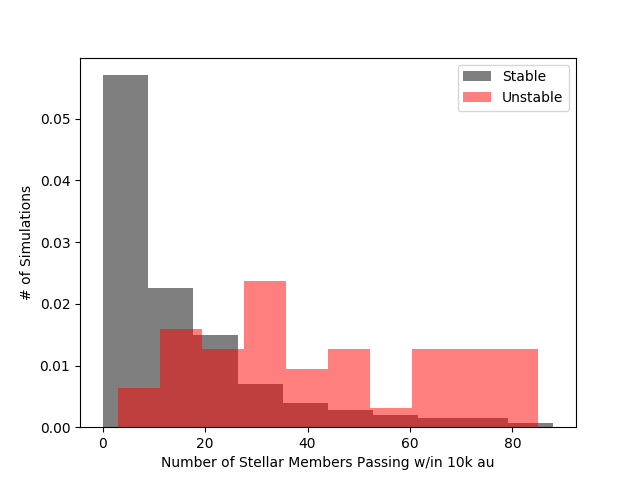
\includegraphics[width=0.5\textwidth]{fig/hist_num_total_stars.png}
    \plottwo{fig/hist_num_total_stars.png}{fig/scatterplot_num_total_stars_nearby_spinorb.png}
    \caption{A normalized histogram containing results from all 3 suites of simulation depicting the distribution of 
    number of 'close' (within 10k au) encounters the planetary system has with cluster stars.}
    \label{fig:close_hist}
\end{figure}
We must also look to the fate of the binary companion. In general, the orbit of a surviving binary companion is not 
closely tied to the orbits of the planets. 
%This is shown in Fig.\ref{fig:ang_correlation}. 
While unstable systems have a preference 
for a high inclination, this is not tied to the inclination of the binary companion. Additionally, we can look to whether or not the binary 
becomes unbound during a simulation. Unstable systems have a nearly $50/50$ split as to whether or not the binary is lost. However, stable systems 
more often than not retain their binary companion. In $93\%$ of systems that keep all 4 planets, the binary remains bound as well. Therefore,
where systems can certainly become unstable with or without the binary staying bound, if a binary does become stripped by the cluster, it is more likely
that 1 or more of the system's planets will also be lost. It is also worth observing that the binary is very likely to survive the cluster overall, so this
architecture of s-type planets with a relatively close binary is quite dynamically stable in the presence of a fully embedded cluster.  
%\begin{figure}
%    \centering
%    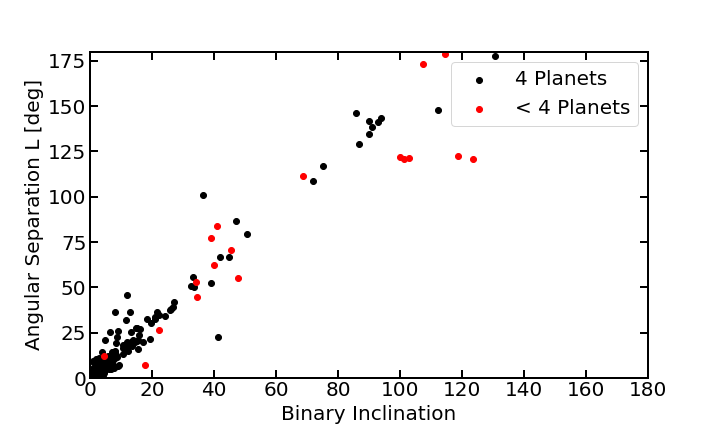
\includegraphics[width=0.5\textwidth]{fig/coupling_scatter_ang_80m.png}
%    \caption{A plot of the angular separation of the angular momentum vector of the binary companion versus the inner planets}
%    \label{fig:ang_correlation}
%\end{figure}
\subsection{Orbital Architecture Changes}
The main takeaway from this project is that the orbital architectures of surviving planets in unstable (lose at least one planet)
 versus stable (retain all four planets) have several noticeable, observable signposts. 
 Primarily, the distributions of eccentricity and the predicted spin-orbit angle of the inner gas giants in 
 unstable systems are statistically distinct from their stable counterparts. High eccentricity planets are thought to have a dynamical source (\cite{dlfm97}).
  We choose to look at the 
 two inner gas giants as they are most likely to survive an instability event and thus act as good markers.
These distributions of the final eccentricity and inclination of the inner giants are shown in Figure \ref{fig:160_ecc_inc}, 
 and a two-sample KS test with an extremely small p-value ($p_{KS} = 1.32e-38$ for the eccentricity distributions
 and $p_{KS} = 1.5e-26$ for the inclinations distributions) shows that we can reasonably infer that they are drawn from different parent distributions. 
\begin{figure}[h!]
    \centering
    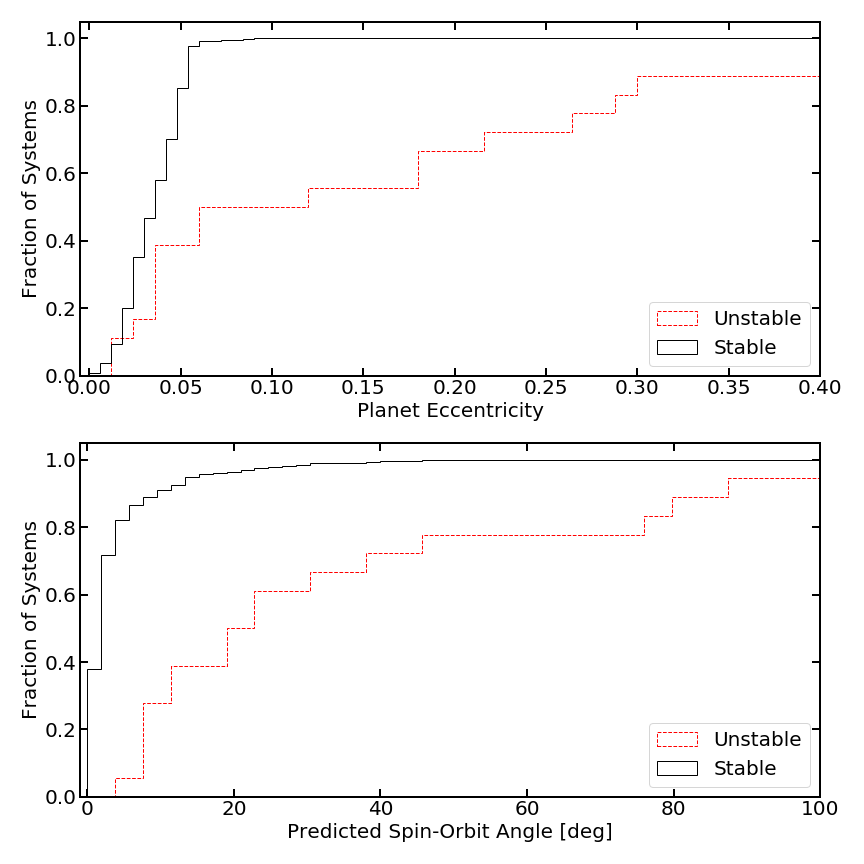
\includegraphics[width=0.5\textwidth]{fig/cumulative_ecc_inc_bigfont80.png}
    
    \plottwo{fig/cumulative_ecc_inc_bigfont160.png}{fig/cumulative_ecc_inc_bigfont341.png}
    \caption{A cumulative distribution depicting the end orbital architectures of planetary systems evolved in a $80M_{\odot}$(top panel), $160M_{\odot}$(bottom left), 
    and $341M_{\odot}$(bottom right) cluster.}
    \label{fig:160_ecc_inc}
\end{figure}
Interactions with the binary companion, whether it remains bound to the primary or not, destabilize the planets via an exchange of orbital 
momentum. If the planets stay bound, this interaction can heat up their orbits to higher eccentricities and inclinations. Often the two
inner planets will undergo a coupled evolution as if in a rigid disk (shown in work by \cite{ina97}), reaching similar inclinations after the instability. 
Additionally, we note that unstable systems are more likely to reach planetary orbits that have \textit{both} high inclination and high eccentricity. This 
sort of pairing of high $\lambda$ and high eccentricity has been seen with Rossiter-McLaughlin observations
(\cite{sch10}) and points to two separate populations: misaligned and aligned with the 
spin of the parent star.
\subsection{Spin Orbit Misalignment \& the birth of Hot Jupiters}
The accepted theory of planet formation is that planets form in a dusty, coplanar circumstellar disk (also called a protoplanetary
disk). A subset of exoplanets that has challenged existing theories of giant planet formation in the field of planetary astrophysics is the 
existence of hot jupiters. Their mode of formation, while debated, is likely very closely tied to their dynamics, 
as their characteristically close position to host stars is not a viable location for in-situ formation. Locations in the disk close to the star
where hot jupiters orbit are likely too hot for gas clouds to collapse due to gravitational instability (\cite{raf05}). As for core accretion in the inner disk,
\cite{lee16} argues that it is unlikely that surface densities are appropriate for in-situ formation of Jupiter mass planets (although they 
and \cite{chi13} note that in-situ super Earth formation.
by core accretion is possible without the need for fine tuning). Therefore, 
the gas giants likely form farther out in the protoplanetary disk and somehow migrate inwards(\cite{lee16},).  This migration can occur in several ways. One is 
smooth migration due to angular momentum exchange with a viscous gaseous disk(\cite{gol80}). \cite{lin96} suggest 
this mechanism for the orbit of famed hot Jupiter 51 Peg b, the first exoplanet discovered orbiting 
a main sequence star \cite{may95}. Smooth disk migration for the case of a single planet is not likely to produce a very eccentric gas giant, as the gas 
disk can dampen high eccentricities(\cite{duf15}). 
The presence of \textit{inclined} hot Jupiters(\cite{alb12}), with their misalignment relative to the Spin
of their host star measure via the Rossiter-McLaughlin effect (\cite{ros24},) further complicates this picture, but also provides more evidence for the dynamical pathway 
of hot jupiter production. 
Other dynamical pathways to produce hot Jupiters include planet-planet scattering, or gravitational interactions with a stellar companion. These mechanisms
have the added effect of forcing gas giants to high eccentricities and/or inclinations. They are of interest to this work due to the preponderance of 
excited planetary orbits among our unstable simulations.\\
%planet-planet
\indent Dynamical instabilities caused by planet-planet scattering can lead to both high eccentricities and high inclinations (\cite{bea12},). Following these scattering events,
the high eccentricities of the gas giants can be damped out by tidal effects (\cite{nag08}), shrinking the orbit and creating a hot Jupiter. \cite{bea12} utilized N-Body 
simulations that include tidal forces. They triggered instabilities by breaking the planets out of an initial resonant configuration.
 The simulations showed that planet-planet encounters and secular effects are the ruling modes of hot Jupiter formation, as opposed to a Kozai resonance. That is,
 the dominant way the hot Jupiters are formed are planets are forced to a low pericenter, high eccentricity orbit by a scattering event, and then are circularized
 by tidal effects. Secular planet-planet interactions can also create a high eccentricity gas giant orbit that can then be circularized. \cite{pet15b} show that this is an 
 efficient process for hot Jupiter formation, but that it does not produce the observed high obliquity sample of misaligned hot Jupiters. \\ 
%planet-binary
\indent Finally, there can be interactions between a planet system and a binary companion.
The binary can exert a torque on either the disk(\cite{bat12}) or a mature planet system (\cite{fab07},\cite{kai11},\cite{dro20}), creating an 
orbital arrangements of a star's planets with high obliquities. Previous work (\cite{fab07})on this topic often points to Kozai-Lidov cycles as the driver of this evolution, 
in which
a sufficiently inclined binary cyclically exchanges angular momentum with a planet and causes it to evolve in eccentricity and inclination. \\
The presence of highly inclined gas giants in our 'unstable' systems
points to a similar pathway to produce these high $\lambda$ exoplanets. Excitement of the binary companion from a stellar cluster
can cause impulsive perturbations (as opposed to longer cyclic Kozai resonances) of planetary systems that result in bound planets with 
high predicted spin-orbit angles.
%To take an in-depth look at inclined, unstable systems, we first want to know if we can treat all 3 suites of simulations' 
%unstable planets as drawn from the same distribution. We should be able to do this, as the mass of the cluster has nothing to 
%do with the interactions between binary and planets once the binary has been excited. Nevertheless, a KS test reveals that we 
%cannot throw out the possibility that all unstable distributions come from the same parent distribution. Thus we will combine 
%all of these simulation results for the following discussion.
%\section{Observing Unstable Systems}
%While we can make a clear distinction between the 'stable' and 'unstable' systems in this numerical experiment,
%it is important to put these systems in the context of exoplanet observations. That is, does the distribution of unstable planet 
%inclinations (a good proxy for the spin-orbit misalignment of the system) make up something that we can observe via the
%Rossiter-McLaughlin effect from a transiting exoplanet.
%We can assume an a-priori distribution of stellar spins as $p(\Psi)=\sin{(\Psi)}$(\cite{fab09}). Drawing from this distribution, 
%we can infer a distribution of observable spin-orbit angles $\lambda$. Drawing from a random spin orientation of the primary star will
%flatten our inclination distribution.
\section{Conclusions and Future Work}
Our initial work has shown that the presence
of cluster stars can have the effect of destabilizing a significant fraction of binary systems by causing the binary companion to migrate closer to the orbiting gas giants.
In particular, we have found that these unstable systems have a significantly different orbital architecture than their stable counterparts. 
%We can make a comparison between our highly inclined unstable systems and the observed population of misaligned hot jupiters. \\
Future work with this integrator includes continuing this experiment with different initial planetary configurations and binary configurations to see how the cluster could
perturb or destabilize these systems. For instance, we will look into varying the eccentricity distribution of the binary companion to pinpoint in parameter space
if there are particular initial conditions more succeptible to destabilization via the cluster environment.
%There has been recent focus on the dynamics of the super-earth system $\pi$ Mensae that is host to two misaligned planets(\cite{hod21}).
%I believe that looking into a numerical experiment with super-earth or sub-neptune planets could have interesting results in  \\
We also have found that in some of our simulations, there seem to be a sprinkling of new binaries and triplet groups of bound stars that form as the cluster evolves. 
Most discussion of stellar multiple formation focuses on fragmentation of dense cores that examines the binary population
at a very early stage(for example \cite{bon94}) and utilize largely smooth particle hydrodynamics, so these simulations could form an interesting dynamical approach to stellar multiple
formation for more mature stellar systems, similar to integrations done in \cite{kro01} and \cite{moe10}. While it is thought that interactions with the primordial gas disk is the ruling
determinant in the orbital architecture of binaries(\cite{kro01,krobur01,bat00}), it would be interesting to see where the small fraction of 
dynamical multiples fit in the parameter space of binary separation and eccentricity. Their survival rates in the presence of their cluster environment will also 
be of interest; that is, we would investiage the question of is the formation of multiples in this fashion a stable pathway.\cite{moe10} examined this question with a hydrodynamic
simulation of an expanding stellar cluster, so the first course of action would be to investigate how the multiples we see fit with prior observations.
\bibliographystyle{aasjournal.bst}
\bibliography{bibliography.bib}
\end{document}